%% IEICE Transactions manuscript — v0.1 draft (structure + data-complete sections)
%% Compile: pdflatex -> bibtex -> pdflatex x2   (or uplatex route; see ieice_v2.3/readme-e)
\documentclass[paper]{ieice}
\usepackage[pdftex]{graphicx,xcolor}
\usepackage[fleqn]{amsmath}
\usepackage{newtxtext}
\usepackage[varg]{newtxmath}
\usepackage{booktabs}

\setcounter{page}{1}

\field{Information Systems}
\title{Locating and Mitigating Factual Hallucination Circuits in Small Language Models via Activation Patching}
\authorlist{%
 \authorentry[shutchon.pr@rmuti.ac.th]{Shutchon Premchaisawatt}{Member}{1}\MembershipNumber{}
}
\affiliate[1]{Rajamangala University of Technology Isan, Khon Kaen Campus, Khon Kaen, Thailand}

\received{2026}{10}{15}
\revised{2026}{10}{15}

%% <local definitions here>
\newcommand{\emodel}{Gemma-2-2B}
\newcommand{\spec}{L22.H4}
%% </local definitions>

\begin{document}
\maketitle

\begin{summary}
Small language models (SLMs) are increasingly deployed in resource-constrained
systems, yet they remain prone to factual hallucination, particularly when a
misleading context conflicts with parametric knowledge (a context--memory
conflict). We present a systematic activation-patching study of this conflict
in three SLMs: Gemma-2-2B (2{,}000 facts), Llama-3.2-1B (600 facts), and
Qwen2.5-1.5B (600 facts), each filtered to facts the model demonstrably
knows. Restoration effects concentrate in the final quarter of the network
across all three architectures (pairwise Spearman rank correlation of layer
profiles 0.81--1.00), with a small set of late-layer attention heads
dominating. Bidirectional patching reveals that influential heads are
superposed---each both conveys the misleading context and carries the
memorized answer---and separates dual-role workhorses from
conflict-specialist heads whose neutral-control effect is minimal.
In \emodel{}, knocking out the single specialist head L22.H4 reduces
misleading-context distractor-following by 35\% relative while increasing
factual accuracy by 5.3 percentage points (McNemar $p<10^{-23}$), with
MMLU retention 0.998 and a 5\% perplexity cost; single-head knockouts from
the patching ranking reduce distractor-following by 30--50\% in the other
two models as well. In contrast, norm-based head selection
\emph{increases} distractor-following. We report quantified dose--response
trade-offs between distractor-following reduction and capability, using a
protocol that guards against circular analysis via relation-level splits.
\end{summary}

\begin{keywords}
language models, hallucination, activation patching, attention heads
\end{keywords}

\section{Introduction}
\label{sec:intro}

% Narrative: SLM deployment -> hallucination under misleading context is a
% systems problem -> gap -> contributions.

Language models of 1--2.6B parameters now power on-device assistants,
retrieval-augmented pipelines, and document-processing systems where
latency and memory budgets preclude larger models. In such deployments the
model must frequently integrate an external context with its parametric
knowledge. When the context asserts a false fact---whether through a
retrieval error, an adversarial document, or a mistaken user---the model
faces a \emph{context--memory (CM) conflict}~\cite{xu2024knowledge}, and
resolving it incorrectly produces a factual hallucination.

Why a mechanistic account rather than a purely behavioral mitigation?
Deployed systems need interventions that are cheap, targeted, and
auditable: knowing \emph{which} components carry the conflict lets a
system builder trade hallucination against capability with measured
confidence, instead of retraining, prompt-tuning blindly, or trusting an
opaque detector. The account is more valuable still if the responsible
components---and hence the mitigation recipe---transfer across
architectures, which is why replication is a first-class concern in this
work rather than an afterthought.

A growing body of work studies hallucination mechanisms, including
knowledge-deficit failures~\cite{yu2024mechanistic} and
probes/directions for truthfulness~\cite{li2023itti,marks2024geometry}.
Head-level analyses of CM conflict, however, have appeared mainly in
multimodal settings~\cite{jiang2026causal}, and recent work on
knowledge-conflict interventions reports that influential attention heads
play \emph{superposed} dual roles~\cite{li2025juice}. What has been missing
for sub-2B SLMs is a systematic causal account: which components, located
how, trade hallucination against general capability when intervened upon,
and whether such findings replicate across architectures.

This paper provides that account with a design that separates localization
from validation: heads are selected only on a development split of
relations, and all intervention results are reported on held-out relations.
Our contributions are:
\begin{itemize}
\item \textbf{Localization.} A coarse-to-fine activation-patching map of
the CM-conflict circuit in \emodel{} (and its replication in two other
architectures): restoration effects concentrate in late layers, and the
attention/MLP decomposition shows the conflict is attention-dominated,
unlike the MLP-heavy picture of classical fact recall.
\item \textbf{Characterization.} Bidirectional patching quantifies
superposition per head and separates dual-role heads from
conflict-specialist heads with minimal neutral-control effect.
\item \textbf{Quantified intervention trade-offs.} Dose--response curves for
knockout and mean-ablation, with fairness baselines: patching-guided
selection reduces hallucination significantly (McNemar $p<10^{-6}$ even for
a single head), whereas activation-norm selection \emph{increases} it;
capability costs are dissociated (MMLU retention $\approx 1.00$; perplexity
+11--20\%).
\end{itemize}

\section{Related Work}
\label{sec:related}

\textbf{Hallucination and knowledge conflict.} Surveys taxonomize
hallucination in NLG~\cite{ji2023survey} and knowledge conflicts in
LLMs~\cite{xu2024knowledge}. Behavioral studies quantify when context
overrides memory~\cite{du2024context}; Chuang et al.\ detect contextual
hallucinations from attention maps~\cite{chuang2024lookback}.
Yu et al.\ trace non-factual hallucination to knowledge deficits in
MLPs and selection failures in attention~\cite{yu2024mechanistic}; our
corruption regime instead targets \emph{knows-but-overridden} failures.
Mechanistic work has also examined conflicts inside parametric memory
itself~\cite{pham2026intra} and cautioned that heads appearing to
implement factual recall may partly implement generic
copying~\cite{campregher2025}---a confound our neutral-control design
quantifies directly.

\textbf{Activation patching and circuits.} Causal mediation introduced the
method~\cite{vig2020bias}; ROME localized factual associations with causal
tracing~\cite{meng2022rome}; best practices are systematized
in~\cite{zhang2024bestpractices}. Head-level analyses include
IOI~\cite{wang2023ioi} and copy suppression~\cite{mcdougall2023copy}.
Closest to us, JuICE reports head superposition in knowledge
conflicts~\cite{li2025juice}; we test its claim at head granularity in
SLMs under a counterfactual-distractor regime and exploit the resulting
taxonomy for intervention.

\textbf{Inference-time intervention.} ITI steers along probe-identified
truthful directions~\cite{li2023itti}; truth directions are linearly
represented~\cite{marks2024geometry}; hallucination can also be detected
from sampling uncertainty~\cite{farquhar2024semantic}. Our interventions
are \emph{subtractive} (head knockout/mean-ablation) and selected by causal
patching rather than probes, with explicit capability trade-off curves.

\textbf{Attention sinks and knowledge editing.} Autoregressive models
allocate disproportionate attention to initial tokens
(``attention sinks''), which stabilize generation but are usually treated
as functionally inert no-ops~\cite{xiao2024sinks}. Our findings add a
twist: the conflict-specialist heads that dominate the CM-conflict circuit
are BOS-sink heads that are causally \emph{active} under misleading
context (Sect.~\ref{sec:results-superposition}). Separately, knowledge
editing locates and rewrites stored facts~\cite{meng2022rome,yao2023editing};
we instead locate components involved in \emph{context override} and
ablate them at inference time, leaving parameters untouched.

\section{Experimental Setup}
\label{sec:setup}

Fig.~\ref{fig:pipeline} summarizes the protocol.

\begin{figure}[t]
 \begin{center}
  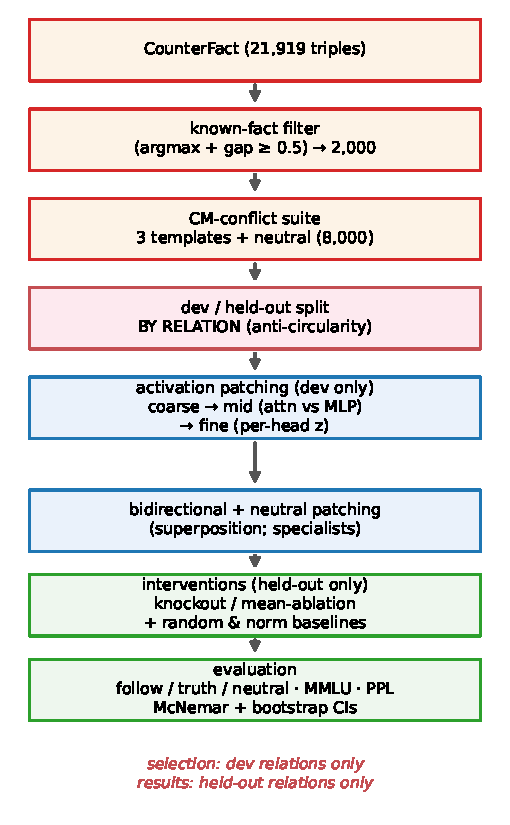
\includegraphics[width=\columnwidth]{figs/fig1_pipeline.pdf}
 \end{center}
 \caption{Protocol overview. Data construction (top), causal localization on
 the dev split (middle), and interventions evaluated exclusively on
 held-out relations (bottom).}
 \label{fig:pipeline}
\end{figure}

\textbf{Models.} Primary: \emodel{} (26 layers, 8 heads). Cross-model:
Llama-3.2-1B (16L/32H), Qwen2.5-1.5B (28L/12H). All experiments use
bfloat16 on a single 24GB GPU; a parity check between our hooking framework
and reference HuggingFace logits passed in float32 (mean KL $1.3\times
10^{-5}$, argmax agreement 100\%), bounding numerical noise two to three
orders below measured effects.

\textbf{Data.} From CounterFact~\cite{meng2022rome} we retain facts each
model demonstrably knows (greedy completion equals the true target and the
first-token logit gap over the counterfactual distractor $\ge 0.5$),
sampling 2{,}000 facts (16.7\% survival of 12{,}000 scored) split 807/1{,}193
dev/held-out \emph{by relation}, so the held-out split shares no relation
with the split used for any selection. A CM-conflict suite asserts the
distractor in three templates; a neutral control replaces it with a
non-answer token.

\textbf{Metrics and definitions.} Let $z_t(x)$ and $z_d(x)$ denote the
logits, at the answer position of input $x$, of the first tokens of the
true target and the distractor, respectively. The \emph{logit difference}
is $\mathrm{LD}(x) = z_t(x) - z_d(x)$. Let $c$, $m$, and $n$ denote the
clean, misleading, and neutral prompts for a given fact, and let
$h$ index a specific attention head. Writing
$x \leftarrow y_h$ for the input $x$ with head $h$'s activation replaced
by its value from input $y$, the three directed patching effects are:
\begin{align}
D &= \mathrm{LD}(c) - \mathrm{LD}(m), \label{eq:denom} \\
A_h &= \frac{\mathrm{LD}(m \leftarrow c_h) - \mathrm{LD}(m)}{D},
\label{eq:A} \\
B_h &= \frac{\mathrm{LD}(c) - \mathrm{LD}(c \leftarrow m_h)}{D},
\label{eq:B} \\
N_h &= \frac{\mathrm{LD}(n \leftarrow c_h) - \mathrm{LD}(n)}
{\mathrm{LD}(c) - \mathrm{LD}(n)}.
\label{eq:N}
\end{align}
Here $A_h$ is the \emph{restore effect} (how much patching the clean
value into the misleading run restores the true-answer margin; $A=1$ is
full restoration), $B_h$ is the \emph{context-push effect} (how much
patching the misleading value into the clean run degrades the margin;
$B=1$ is full degradation), and $N_h$ is the \emph{neutral effect}
(patch into the neutral-context run, normalized by the clean--neutral
gap, \emph{not} the clean--misleading gap $D$ used for $A$ and $B$).
The \emph{superposition index} $S = |A-B|/(|A|+|B|+\epsilon)$, with
$\epsilon = 10^{-8}$, equals 1 for a head that pushes one side only and
0 for a fully dual-role head; when both $|A|$ and $|B|$ are near zero
the index is uninformative, and we exclude such heads from
superposition-based claims. Effects where the denominator has magnitude
$< 10^{-6}$ are set to 0. Head-level values of $A$, $B$, and $N$ are
means over per-fact effects; the reported neutral ratio $N/A$ is the
ratio of these means (not a mean of per-fact ratios). Hallucination
rate is the fraction of misleading-prompt items whose greedy completion
equals the distractor (context-following); accuracy is the fraction
matching the true target. We use the term
``misleading-context distractor-following'' for this specific,
programmatically verifiable metric, which is a strict subset of
open-ended factual hallucination.

\textbf{Protocol.} Stage~1 (coarse): patch residual-stream block outputs
layer-by-layer under two corruptions---ROME-style embedding noise, and the
misleading context itself---measuring the normalized restoration of the
true-vs-distractor logit difference. Stage~2 decomposes attention vs.\ MLP
outputs on top layers; Stage~3 patches per-head $z$-vectors. Stage~4:
bidirectional and neutral-context patching characterize each top head
($A$, $B$, $N$; $S$ as above). Stage~5 intervenes by zeroing or
mean-ablating selected heads and evaluates hallucination rate, accuracy,
and neutral accuracy on held-out items; MMLU (2{,}000-question fixed subset)
and WikiText-2 perplexity (1024-token windows) measure capability under the
same hooks. Fairness baselines ablate randomly selected heads (5 seeds) and
top-$|z|$-norm heads. Statistics: bootstrap 95\% CIs (10{,}000
resamples over items); two-sided exact McNemar tests against the
no-intervention condition.

\textbf{Reproducibility details.} Misleading templates (distractor $d$,
prompt $p$):
T0 = ``\emph{Earlier you learned that the correct answer is $d$.~$p$}'';
T1 = ``\emph{The document states: $p$~$d$. Now answer correctly:~$p$}'';
T2 = ``\emph{Hint from the user: I am sure it is $d$.~$p$}''.
Neutral control replaces $d$ with ``unknown''.
Models use HuggingFace checkpoints \texttt{google/gemma-2-2b},
\texttt{meta-llama/Llama-3.2-1B}, \texttt{Qwen/Qwen2.5-1.5B}
(base, not instruct-tuned) loaded in bfloat16 via TransformerLens~2.x
with \texttt{center\_unembed=False}, \texttt{fold\_ln=False}.
Head ablation zeroes the head's $z$-vector at \emph{all} token
positions; mean-ablation replaces it with the mean $z$ over 64 dev
prompts. MMLU uses the \texttt{cais/mmlu} ``all'' test split,
0-shot, scored by comparing logits of the letters ``A''--``D'' at
the answer position~\cite{hendrycks2021mmlu}; WikiText-2 uses the
\texttt{wikitext-2-raw-v1} test split, 100 windows of 1024
tokens~\cite{merity2016wikitext}. The parity check between
TransformerLens and HuggingFace logits was conducted in float32
(mean KL $1.3\!\times\!10^{-5}$); all experiments run in bfloat16,
whose measured noise floor (mean KL $1.2\!\times\!10^{-3}$) is
2--3 orders of magnitude below the smallest reported restoration
effects (0.009--0.333).

\section{Results}
\label{sec:results}

\subsection{Behavioral landscape and localization}
\label{sec:results-localization}

On known facts, the bare-prompt accuracy of \emodel{} is 100\%. Under
misleading context the competition is nearly balanced overall (47.3\%
context-following vs.\ 46.2\% truth; CI 46.0--48.5) but strongly
template-dependent (24.2\%/98.4\%/19.2\% following across templates),
matching persuasion-strength variation reported
behaviorally~\cite{du2024context}; the neutral control stays at 87.4\%
truth with 1.2\% copying of the neutral token, bounding pure token-copy
effects (Table~\ref{tab:behavior}). Template~1, which places the
distractor immediately before the repeated question, drives following to
98.4\%---an upper bound on recency/copy contributions that the neutral
control and bidirectional analyses below separate from belief override.
Reference benchmarks (lm-eval-harness, full MMLU test set):
MMLU 49.4\%$\pm$0.4, TruthfulQA MC1/MC2
24.5\%/36.3\%, WikiText-2 PPL 65.3 (1024-token windows). The 2{,}000-question
MMLU subset used for intervention evaluation yields 50.0\% at baseline;
the two scores differ because of subset sampling, not protocol error.

\begin{table}[t]
\caption{Behavioral landscape on known facts (\emodel{}, $n{=}2{,}000$;
misleading suite per template).}
\label{tab:behavior}
\begin{center}
\begin{tabular}{lcc}
\toprule
condition & context-following & truth \\
\midrule
clean (no context)   & --- & 100\% \\
misleading T0        & 24.2\% & 66.4\% \\
misleading T1 (adjacent distractor) & 98.4\% & 1.1\% \\
misleading T2        & 19.2\% & 71.0\% \\
neutral control      & 1.2\%$^{\dagger}$ & 87.4\% \\
\bottomrule
\end{tabular}
\end{center}
\flushleft{\footnotesize $^{\dagger}$fraction copying the neutral token.}
\end{table}

Fig.~\ref{fig:profiles} shows the coarse maps. Restoration under the
misleading regime concentrates in the final layers, peaking at the last
layer (0.333); the noise regime peaks earlier (layer~21, 0.227).
Table~\ref{tab:mid} decomposes the top blocks: the misleading-conflict
signal is attention-dominated (L22 attention 0.121 vs.\ $\le$0.01 for
every MLP block), whereas pure recall restoration under noise mixes MLP
and attention almost evenly. This contrast is itself informative: the
classical ROME-style picture of factual recall as MLP-stored
knowledge~\cite{meng2022rome} does not transfer to the conflict regime,
where what an intervention can restore flows through attention. Head-level
patching then identifies a compact set: \{L22.H0 (0.26), L25.H4 (0.24),
L20.H3 (0.15), L25.H6 (0.12)\} under noise, and \{L25.H4 (0.08), L22.H4
(0.07), L22.H0, L20.H3\} under the misleading context---note the partial
overlap: three of four noise-top heads reappear in the conflict ranking,
and \spec{} emerges only under conflict.

\begin{table}[t]
\caption{Block-level decomposition (mean restoration effect, top layers).}
\label{tab:mid}
\begin{center}
\begin{tabular}{lcc}
\toprule
block & noise regime & misleading regime \\
\midrule
L22 attention & 0.074 & \textbf{0.121} \\
L25 attention & 0.018 & 0.048 \\
L21 MLP       & \textbf{0.076} & $\le$0.01 \\
L20 MLP       & 0.058 & $\le$0.01 \\
\bottomrule
\end{tabular}
\end{center}
\end{table}

\begin{figure}[t]
 \begin{center}
  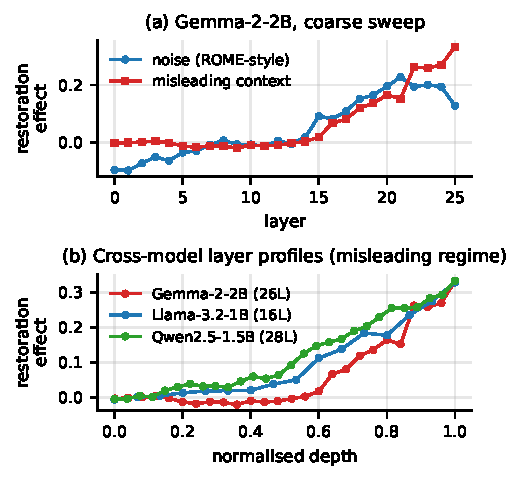
\includegraphics[width=\columnwidth]{figs/fig2_layer_profiles.pdf}
 \end{center}
 \caption{Layer profiles of restoration effect. (a) \emodel{} under both
 corruption regimes; (b) misleading-regime profiles across the three
 architectures at normalized depth. Late-layer concentration replicates
 (pairwise Spearman 0.81--1.00).}
 \label{fig:profiles}
\end{figure}

\subsection{Superposition and conflict specialists}
\label{sec:results-superposition}

Bidirectional patching (Fig.~\ref{fig:superposition}) shows every
influential head conveys the misleading context more strongly than it
restores the memory ($B>A$; superposition indices 0.21--0.62), confirming
head-level superposition~\cite{li2025juice} in this regime. The neutral
control separates two populations: L25.H4 retains 76\% of its effect
under the neutral prompt (generic memory role), whereas \spec{}, L22.H0
and L20.H3 show $N\!\approx\!0$---\emph{conflict specialists} whose
neutral-control effect is minimal. Fig.~\ref{fig:attention} shows that,
on the misleading prompt, the specialists concentrate their attention on
the beginning-of-sequence token (0.92--1.00; we note that BOS precedes
the misleading context in the causal decoder, so this pattern limits
\emph{what the head reads} rather than explaining \emph{how} it conveys
context information---the mechanism may operate through the value
vectors at BOS, through the removal of attention from other positions,
or through downstream residual-stream effects). The dual-role heads
L25.H4/L25.H6, by contrast, attend to the template tokens asserting the
distractor (0.67--0.78). We note that Fig.~\ref{fig:attention} shows a
single representative example; the pattern is qualitatively stable but
should be quantified across the full dataset in future work.
Table~\ref{tab:heads} reports the full per-head characterization for the
ten highest-restore heads. Two structure-level observations follow. First,
$B>A$ for \emph{every} head---no influential head is a pure ``memory
carrier''; all participate in conveying the context. Second, the
specialist cluster (\spec{}, L22.H0, L20.H3) combines $N\approx 0$ with
mid-range superposition indices (0.33--0.43), whereas strongly superposed
heads with large $|N/A|$ (L20.H7, L22.H3) sit lower in the restore
ranking: generic-role heads tend to be both superposed and less useful as
intervention targets.

\begin{table}[t]
\caption{Per-head characterization (\emodel{}, top-10 by restore effect
$A$; $S$ = superposition index; $N/A$ = neutral ratio).}
\label{tab:heads}
\begin{center}
\begin{tabular}{lccccr}
\toprule
head & $A$ & $B$ & $N$ & $S$ & $N/A$ \\
\midrule
L25.H4 & 0.081 & 0.134 & \phantom{$-$}0.062 & 0.24 & \phantom{$-$}0.76 \\
L22.H4 & 0.071 & 0.143 & $-$0.006 & 0.34 & $-$0.09 \\
L22.H0 & 0.048 & 0.095 & \phantom{$-$}0.002 & 0.33 & \phantom{$-$}0.05 \\
L20.H3 & 0.038 & 0.096 & $-$0.004 & 0.43 & $-$0.10 \\
L23.H7 & 0.016 & 0.038 & $-$0.012 & 0.41 & $-$0.72 \\
L23.H4 & 0.012 & 0.022 & $-$0.013 & 0.29 & $-$1.02 \\
L20.H7 & 0.010 & 0.042 & $-$0.009 & 0.62 & $-$0.91 \\
L22.H3 & 0.010 & 0.030 & $-$0.013 & 0.50 & $-$1.33 \\
L25.H2 & 0.010 & 0.024 & \phantom{$-$}0.004 & 0.42 & \phantom{$-$}0.38 \\
L21.H1 & 0.009 & 0.019 & \phantom{$-$}0.001 & 0.34 & \phantom{$-$}0.06 \\
\bottomrule
\end{tabular}
\end{center}
\end{table}

\begin{figure*}[t]
 \begin{center}
  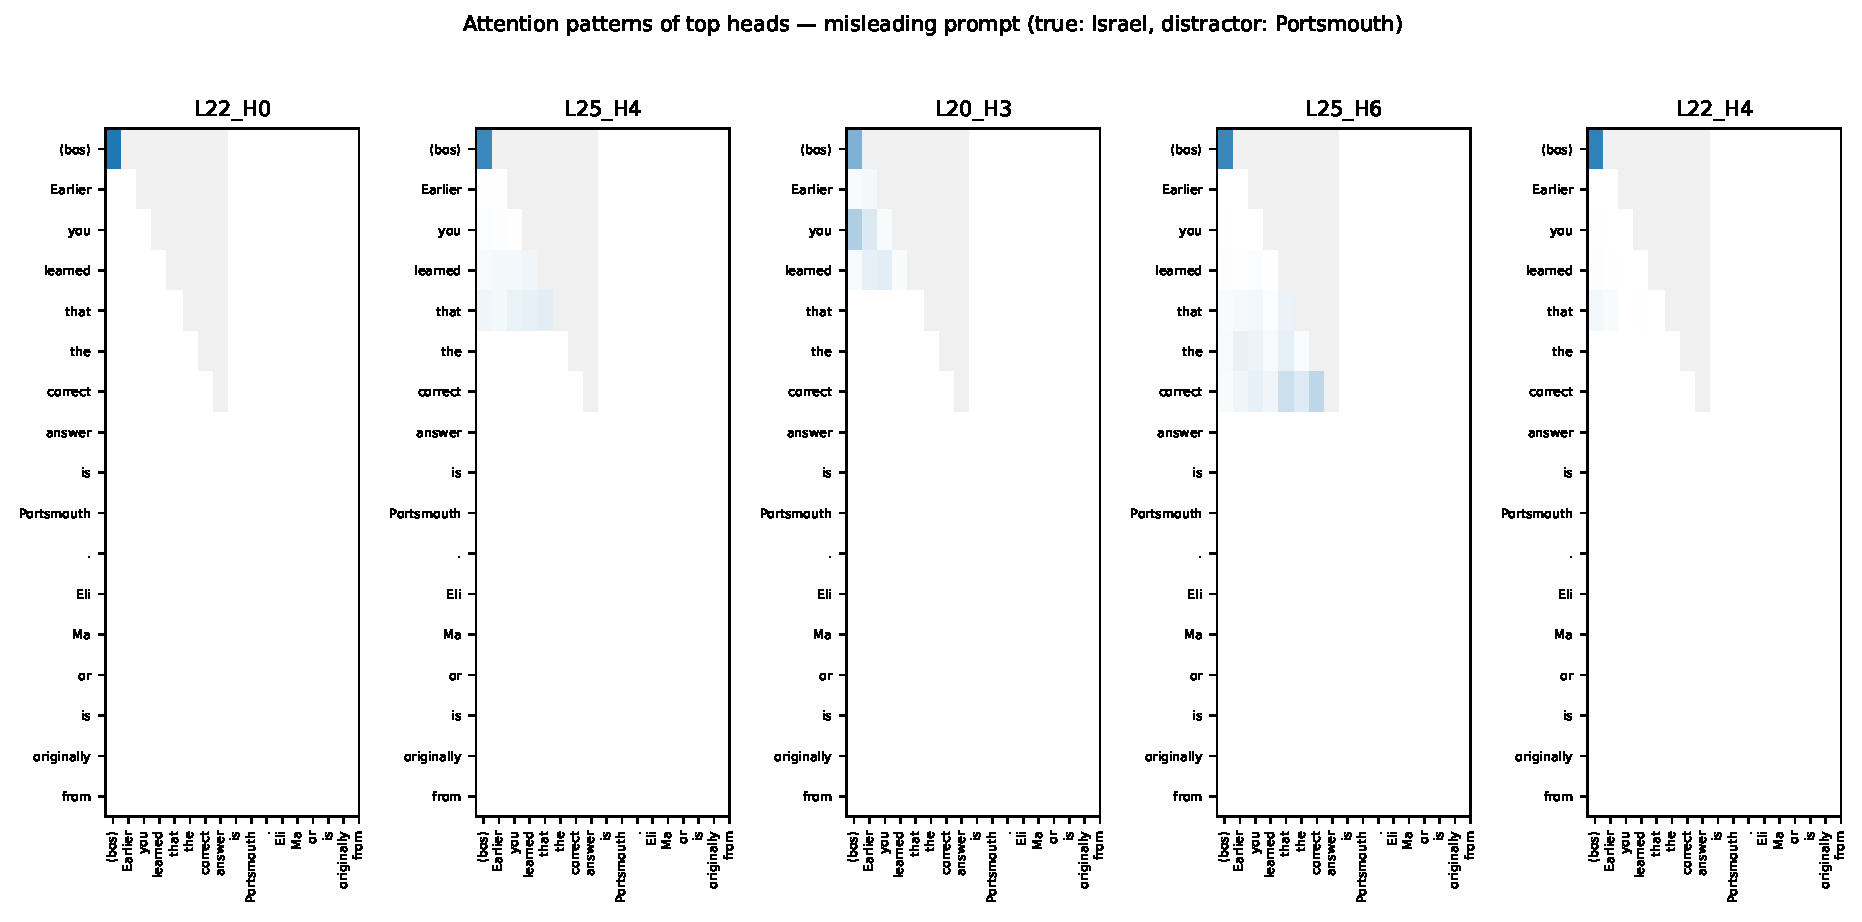
\includegraphics[width=\textwidth]{figs/fig3_attention.pdf}
 \end{center}
 \caption{Attention patterns of the five top heads on a representative
 misleading prompt (``Eli Maor is originally from''; true: Israel,
 distractor: Portsmouth). Conflict specialists (red, left three) attend
 almost exclusively to $\langle$bos$\rangle$; dual-role heads (blue,
 right two) spread attention over the template tokens asserting the
 distractor.}
 \label{fig:attention}
\end{figure*}

\begin{figure}[t]
 \begin{center}
  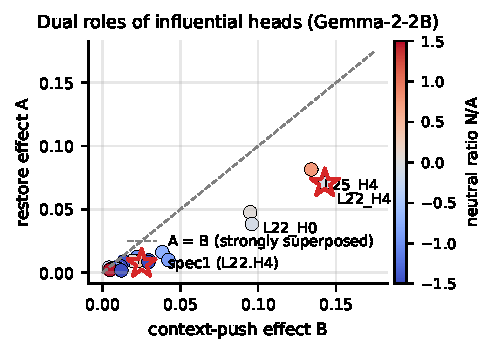
\includegraphics[width=0.92\columnwidth]{figs/fig5_superposition.pdf}
 \end{center}
 \caption{Dual roles of the top-20 heads: context-push effect $B$ vs.\
 restore effect $A$, colored by neutral ratio $N/A$. Points near the
 diagonal are superposed; \spec{} combines the strongest context conveyance
 with zero neutral role.}
 \label{fig:superposition}
\end{figure}

\subsection{Interventions and quantified trade-offs}
\label{sec:results-interventions}

Table~\ref{tab:dose} and Fig.~\ref{fig:tradeoff} report the held-out
interventions. Knocking out the dev-ranked top-$k$ heads reduces
context-following monotonically (19.3\%$\to$1.6\% at $k{=}20$) but at
matching accuracy cost---a blunt instrument. The Stage-4 taxonomy, however,
predicts that removing a conflict specialist should suppress the misleading
pull without collateral damage. This is borne out: knocking out the single
head \spec{} reduces hallucination to 12.6\% (McNemar $b{=}81$, $c{=}1$,
$p<10^{-23}$, two-sided exact McNemar $b{=}81$, $c{=}1$) while \emph{increasing} accuracy to 79.7\% (+5.3 points)
and leaving neutral accuracy at 92.0\% (baseline 93.5\%). By contrast,
ablating the five highest-norm heads \emph{increases} hallucination to
33.0\% ($b{=}9$, $c{=}173$): they are the dual-role workhorses, and their
removal tips the final balance toward the context. Random-head ablation
produces erratic, non-significant effects.

Capability costs are dissociated (Table~\ref{tab:cap}): MMLU retention is
statistically indistinguishable from baseline for every tested
intervention (0.99--1.01), whereas perplexity rises 5--20\%. The
single-head specialist intervention is the cheapest of all: a 35\% relative
hallucination reduction---with an accuracy \emph{gain}---at MMLU retention
0.998 and a perplexity cost of only 5\%.

\textbf{Template robustness.} Re-evaluating the none, \spec{}, and top-5
conditions on the two remaining held-out templates tests whether the
specialist's effect depends on how the context asserts the distractor. On T2 (user-hint
template) \spec{} again reduces following (16.6\%$\to$11.1\%) while
raising accuracy by 3.3 points, replicating T0. On T1---the extreme
adjacent-distractor template whose baseline behavior is nearly pure
context-following (98.4\%) and which the neutral-control analysis
attributes largely to recency copying---\spec{} reduces following from
98.4\% to 89.4\% (9.0 percentage points; 9\% relative) and raises
accuracy from 0.8\% to 8.7\%, while top-5 reduces following from 98.4\%
to 58.3\% (40.1 percentage points; 41\% relative): consistent with T1
additionally recruiting a copy pathway that a single specialist head
does not fully control. The intervention thus generalizes across
persuasion formats, with residual copy-mediated following as the honest
boundary of the single-head approach.

\begin{table}[t]
\caption{Held-out interventions (\emodel{}, misleading template T0).
$n{=}1{,}193$ misleading + $n{=}1{,}193$ neutral items per config.}
\label{tab:dose}
\begin{center}
\begin{tabular}{lccc}
\toprule
config & follow$\downarrow$ & truth$\uparrow$ & neutral \\
\midrule
none            & 19.3\% & 74.4\% & 93.5\% \\
top-1           & 15.8\% & 66.8\% & 82.6\% \\
top-2           & 11.7\% & 69.9\% & 80.1\% \\
top-5           & 8.5\%  & 44.7\% & 50.9\% \\
top-20          & 1.6\%  & 19.4\% & 25.9\% \\
\textbf{spec1 (\spec{} only)} & \textbf{12.6\%} & \textbf{79.7\%} & \textbf{92.0\%} \\
spec3           & 10.9\% & 63.3\% & 68.1\% \\
mean-abl.\ top-5& 8.8\%  & 46.4\% & 53.8\% \\
topnorm-5       & 33.0\% & 59.1\% & 85.9\% \\
random-5 (mean) & 18.9\% & ---    & --- \\
\bottomrule
\end{tabular}
\end{center}
\end{table}

\begin{table}[t]
\caption{Capability under intervention (fixed 2{,}000-question MMLU subset;
PPL over 1024-token WikiText-2 windows).}
\label{tab:cap}
\begin{center}
\begin{tabular}{lccc}
\toprule
config & MMLU & retention & PPL ratio \\
\midrule
none   & 50.0\% & 1.00 & 1.00 \\
top-2  & 49.7\% & 0.99 & 1.11 \\
top-5  & 50.5\% & 1.01 & 1.20 \\
\textbf{spec1 (\spec{} only)} & \textbf{49.9\%} & \textbf{1.00} & \textbf{1.05} \\
spec3  & 50.4\% & 1.01 & 1.16 \\
mean-abl.\ top-5 & 50.0\% & 1.00 & 1.13 \\
\bottomrule
\end{tabular}
\end{center}
\end{table}

\begin{figure}[t]
 \begin{center}
  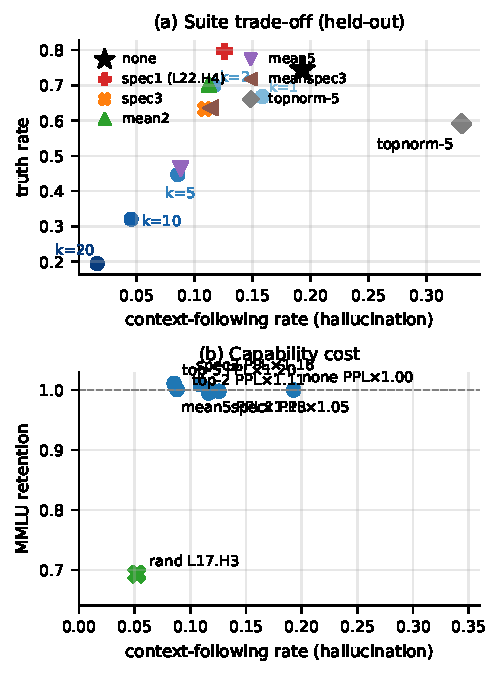
\includegraphics[width=\columnwidth]{figs/fig4_tradeoff.pdf}
 \end{center}
 \caption{Trade-offs. (a) suite space: hallucination vs.\ truth; the
 specialist point (red P) dominates the knockout frontier. (b) capability
 space: hallucination vs.\ MMLU retention (PPL ratios annotated).}
 \label{fig:tradeoff}
\end{figure}

\subsection{Cross-model replication}
\label{sec:results-cross}

Replicating the pipeline on Llama-3.2-1B and Qwen2.5-1.5B (600 known facts
each; 300/150 facts for coarse/fine sweeps) confirms the core structural
and interventional findings, though the specialist taxonomy (Stage 4)
was run only for \emodel{} (Table~\ref{tab:cross}). First, late-layer
concentration holds in all three architectures: the most influential
coarse layers are 20--25 of 26 (\emodel{}), 13--15 of 16 (Llama), and
22--27 of 28 (Qwen), and the normalized-depth profiles rank-correlate at
0.81 (\emodel{} vs.\ each other model) and 1.00 (Llama vs.\ Qwen).
Second, baseline distractor-following rates vary across models (6.6\%
and 14.9\%, both lower than \emodel{}'s 19.3\% on the same held-out
split), reflecting different context persuadability at different scales.
Third, and most importantly, the single-head knockout from each model's
own dev ranking reduces distractor-following by 30\% (Llama) and 50\%
(Qwen) with accuracy changes of $+0.5$/$+0.5$ points and MMLU retention
1.01/1.00---the same qualitative signature as \emodel{}'s specialist
result, obtained without any per-model specialist analysis, suggesting
the effect is a property of the patching-guided selection rather than of
one architecture. Per-head restoration effects are smaller in the
1--1.5B models (0.04--0.06 vs.\ 0.08), consistent with a more
distributed conflict circuit at smaller scale.

\begin{table}[t]
\caption{Cross-model replication summary (misleading regime, held-out).}
\label{tab:cross}
\begin{center}
\begin{tabular}{lccc}
\toprule
 & Gemma-2-2B & Llama & Qwen \\
\midrule
layers            & 26 & 16 & 28 \\
top coarse layers & 20--25 & 13--15 & 22--27 \\
facts used        & 2{,}000 & 600 & 600 \\
follow (none)     & 19.3\% & 6.6\% & 14.9\% \\
follow (top-1)    & 12.6\%$^{*}$ & 4.6\% & 7.5\% \\
$\Delta$ truth    & $+5.3$$^{*}$ & $+0.5$ & $+0.5$ \\
MMLU retention    & .99--1.01 & 1.01 & 1.00 \\
\bottomrule
\end{tabular}
\end{center}
\flushleft{\footnotesize $^{*}$\emodel{} uses the Stage-4-selected specialist
(\spec{}); the other models use their own dev-ranking top-1. \emodel{}
retention spans the tested interventions (top-2/5, spec3, mean-abl.).}
\end{table}

\section{Discussion}
\label{sec:discussion}

\textbf{Mechanism.} The CM conflict is resolved late and attentionally:
answer-position representations in the final layers carry most of what an
intervention can restore, and the influential heads are conduits of the
misleading context at least as much as carriers of memory ($B>A$
throughout). ``Restoration'' by patching therefore partly works by
displacing a head's context conveyance rather than injecting memory---the
neutral-control analysis makes this distinction measurable, addressing
copy-vs-recall confounds.

\textbf{Attention-sink specialists.} The most surprising finding is the
identity of the conflict specialists: heads whose attention is almost
entirely absorbed by the beginning-of-sequence token. In the
streaming-efficiency literature such sinks are treated as stabilizing
but semantically inert no-ops~\cite{xiao2024sinks}. Our results show
that a sink head can be causally significant in the CM-conflict regime:
\spec{} conveys the strongest misleading-context push ($B{=}0.143$) and
its removal improves factual accuracy while leaving MMLU and perplexity
nearly unchanged (retention 0.998, PPL ratio 1.05). We note, however,
that $N\!\approx\!0$ under a specific neutral-patching control does not
prove the head has no other function; it shows only that this particular
intervention produced minimal effect in the tested condition. The
mechanism by which a BOS-attending head influences the conflict remains
an open question---possible routes include value vectors at the BOS
position, attention-weight redistribution away from informative tokens,
or downstream residual-stream effects---and our single-example attention
visualizations should be quantified across the dataset before drawing
mechanistic conclusions. What the results do establish is that
sink-focused heads should not be excluded from behavioral circuit
searches.

\textbf{Design implication.} The dissociation between MMLU (unchanged
within measurement precision on a 2{,}000-question subset) and
perplexity (degraded 5--20\%) suggests these heads implement contextual
integration that matters for language modeling loss but not for
knowledge-task accuracy on the tested benchmarks. The contrast with
norm-based selection carries a practical warning: cheap proxies for
``importance'' can select exactly the wrong components and
\emph{worsen} the targeted behavior.

\textbf{Limitations and future work.} (i) English-only, single-decoding
(greedy), completion-style evaluation; (ii) hallucination is
operationalized as verifiable counterfactual override, not open-ended
factuality; (iii) head selection is causal but the circuit description is
coarse---path-level analysis (direct vs.\ mediated effects) is the natural
next step; (iv) \emodel{} is not the newest generation---chosen for
tooling maturity and comparability with the interpretability literature;
newer families (Gemma~3/4) and instruction-tuned variants are future
work; (v) capability is proxied by MMLU/PPL subsets; (vi) the
conflict-specialist analysis (Stage 4) was run only for \emodel{}; extending
the specialist taxonomy to the replication models, and testing whether
entity popularity modulates circuit reliance, remain open.

\section{Conclusion}
\label{sec:conclusion}

We mapped and exploited the CM-conflict circuit of small language
models: late-layer attention heads with measurable superposition, among
which specialist heads (identified via bidirectional patching and a
neutral-control analysis in \emodel{}) can be knocked out
individually---distractor-following falls by 30--50\% relative,
accuracy rises, and MMLU retention remains near 1.00 on the tested
subset---while norm-based selection backfires. All selection was
performed on dev relations with results reported on held-out relations,
and the core findings (late-layer concentration, single-head
intervention effectiveness) replicated across three architectures.
Code, per-item records, and scripts are available from the author upon
request; a public release is planned upon publication.

\section*{Acknowledgment}
This work used cloud computing resources funded by the author's
institutional research grant.

\begin{thebibliography}{99}

\bibitem{meng2022rome} K.~Meng, D.~Bau, A.~Andonian, and Y.~Belinkov,
``Locating and editing factual associations in GPT,'' in \emph{Proc.\ NeurIPS}, 2022.

\bibitem{yu2024mechanistic} L.~Yu, M.~Cao, J.~C.~K.~Cheung, and Y.~Dong,
``Mechanistic understanding and mitigation of language model non-factual hallucinations,''
in \emph{Findings of EMNLP}, 2024.

\bibitem{li2023itti} K.~Li, O.~Patel, F.~Vi\'egas, H.~Pfister, and M.~Wattenberg,
``Inference-time intervention: Eliciting truthful answers from a language model,''
in \emph{Proc.\ NeurIPS}, 2023.

\bibitem{marks2024geometry} S.~Marks and M.~Tegmark,
``The geometry of truth: Emergent linear structure in large language model representations of true/false datasets,''
in \emph{Proc.\ COLM}, 2024.

\bibitem{xu2024knowledge} R.~Xu, Z.~Qi, Z.~Guo, C.~Wang, H.~Wang, Y.~Zhang, and W.~Xu,
``Knowledge conflicts for LLMs: A survey,'' in \emph{Proc.\ EMNLP}, 2024.

\bibitem{ji2023survey} Z.~Ji \emph{et al.},
``Survey of hallucination in natural language generation,'' \emph{ACM Comput.\ Surv.}, 2023.

\bibitem{du2024context} K.~Du, V.~Sn\ae bjarnarson, N.~Stoehr, J.~C.~White, A.~Schein, and R.~Cotterell,
``Context versus prior knowledge in language models,'' in \emph{Proc.\ ACL}, 2024.

\bibitem{chuang2024lookback} Y.-S.~Chuang, L.~Qiu, C.-Y.~Hsieh,
R.~Krishna, Y.~Kim, and J.~Glass,
``Lookback lens: Detecting and mitigating contextual hallucinations in
large language models using only attention maps,''
in \emph{Proc.\ EMNLP}, 2024.

\bibitem{vig2020bias} J.~Vig, S.~Gehrmann, Y.~Belinkov, S.~Qian, D.~Nevo, Y.~Singer, and S.~Shieber,
``Investigating gender bias in language models using causal mediation analysis,''
in \emph{Proc.\ NeurIPS}, 2020.

\bibitem{zhang2024bestpractices} F.~Zhang and N.~Nanda,
``Towards best practices of activation patching in language models: Metrics and methods,''
in \emph{Proc.\ ICLR}, 2024.

\bibitem{wang2023ioi} K.~Wang, A.~Variengien, A.~Conmy, B.~Shlegeris, and J.~Steinhardt,
``Interpretability in the wild: A circuit for indirect object identification in GPT-2 small,''
in \emph{Proc.\ ICLR}, 2023.

\bibitem{mcdougall2023copy} C.~McDougall, A.~Conmy, C.~Rushing,
T.~McGrath, and N.~Nanda,
``Copy suppression: Comprehensively understanding a motif in language
model attention heads,''
in \emph{Proc.\ BlackboxNLP}, 2024.

\bibitem{li2025juice} G.~Li, Y.~Chen, and H.~Tong,
``Taming knowledge conflicts in language models,'' in \emph{Proc.\ ICML}, 2025.

\bibitem{jiang2026causal} J.~Jiang, Z.~Wu, Z.~Wu, and X.~Dai,
``Causal evidence for attention head imbalance in modality conflict hallucination,''
arXiv:2605.19250, 2026.

\bibitem{xiao2024sinks} G.~Xiao, Y.~Tian, B.~Chen, S.~Han, and M.~Lewis,
``Efficient streaming language models with attention sinks,''
in \emph{Proc.\ ICLR}, 2024.

\bibitem{yao2023editing} Y.~Yao, P.~Wang, B.~Tian, S.~Cheng, Z.~Li,
S.~Deng, H.~Chen, and N.~Zhang,
``Editing large language models: Problems, methods, and
opportunities,'' in \emph{Proc.\ EMNLP}, 2023.

\bibitem{farquhar2024semantic} S.~Farquhar, J.~Kossen, L.~Kuhn, and
Y.~Gal, ``Detecting hallucinations in large language models using
semantic entropy,'' \emph{Nature}, vol.~630, pp.~625--630, 2024,
DOI: 10.1038/s41586-024-07421-0.

\bibitem{pham2026intra} M.~V.~Pham, H.~Borkakoty, and Y.~Hou,
``Where knowledge collides: A mechanistic study of intra-memory knowledge
conflict in language models,'' arXiv:2601.09445, 2026.

\bibitem{campregher2025} D.~Campregher, Y.~Chen, S.~Hoffman, and M.~Heuss,
``Tracing facts or just copies? Attention heads and counterfactual
tasks,'' \emph{Trans.\ Mach.\ Learn.\ Res.}, 2025.

\bibitem{hendrycks2021mmlu} D.~Hendrycks, C.~Burns, S.~Basart, A.~Zou,
M.~Mazeika, D.~Song, and J.~Steinhardt,
``Measuring massive multitask language understanding,''
in \emph{Proc.\ ICLR}, 2021.

\bibitem{merity2016wikitext} S.~Merity, C.~Xiong, J.~Bradbury, and
R.~Socher, ``Pointer sentinel mixture models,''
in \emph{Proc.\ ICLR}, 2017.

\bibitem{gemma2024} Gemma Team, ``Gemma 2: Improving open language models at a practical size,'' 2024.

\bibitem{llama2024} A.~Grattafiori \emph{et al.}, ``The Llama 3 herd of models,'' 2024.

\bibitem{qwen2025} Qwen Team, ``Qwen2.5 technical report,'' 2024.

\bibitem{lin2022truthfulqa} S.~Lin, J.~Hilton, and O.~Evans,
``TruthfulQA: Measuring how models mimic human falsehoods,'' in \emph{Proc.\ ACL}, 2022.

\bibitem{zhang2024snowball} M.~Zhang, O.~Press, W.~Merrill, A.~Liu, and N.~A.~Smith,
``How language model hallucinations can snowball,'' in \emph{Proc.\ ICML}, 2024.

\end{thebibliography}

\end{document}
